%% Copernicus Publications Manuscript Preparation Template for LaTeX Submissions
%% ---------------------------------
%% This template should be used for copernicus.cls
%% The class file and some style files are bundled in the Copernicus Latex Package, which can be downloaded from the different journal webpages.
%% For further assistance please contact Copernicus Publications at: production@copernicus.org
%% https://publications.copernicus.org/for_authors/manuscript_preparation.html


%% Please use the following documentclass and journal abbreviations for discussion papers and final revised papers.


%% 2-column papers and discussion papers
\documentclass[acp, manuscript]{copernicus}



%% Journal abbreviations (please use the same for discussion papers and final revised papers)

% Archives Animal Breeding (aab)
% Atmospheric Chemistry and Physics (acp)
% Advances in Geosciences (adgeo)
% Advances in Statistical Climatology, Meteorology and Oceanography (ascmo)
% Annales Geophysicae (angeo)
% ASTRA Proceedings (ap)
% Atmospheric Measurement Techniques (amt)
% Advances in Radio Science (ars)
% Advances in Science and Research (asr)
% Biogeosciences (bg)
% Climate of the Past (cp)
% Drinking Water Engineering and Science (dwes)
% Earth System Dynamics (esd)
% Earth Surface Dynamics (esurf)
% Earth System Science Data (essd)
% Fossil Record (fr)
% Geographica Helvetica (gh)
% Geoscientific Instrumentation, Methods and Data Systems (gi)
% Geoscientific Model Development (gmd)
% Hydrology and Earth System Sciences (hess)
% History of Geo- and Space Sciences (hgss)
% Journal of Micropalaeontology (jm)
% Journal of Sensors and Sensor Systems (jsss)
% Mechanical Sciences (ms)
% Natural Hazards and Earth System Sciences (nhess)
% Nonlinear Processes in Geophysics (npg)
% Ocean Science (os)
% Proceedings of the International Association of Hydrological Sciences (piahs)
% Primate Biology (pb)
% Scientific Drilling (sd)
% SOIL (soil)
% Solid Earth (se)
% The Cryosphere (tc)
% Web Ecology (we)
% Wind Energy Science (wes)


%% \usepackage commands included in the copernicus.cls:
%\usepackage[german, english]{babel}
\usepackage{tabularx}
%\usepackage{cancel}
%\usepackage{multirow}
%\usepackage{supertabular}
%\usepackage{algorithmic}
%\usepackage{algorithm}
%\usepackage{amsthm}
%\usepackage{float}
%\usepackage{subfig}
%\usepackage{rotating}


\begin{document}

\title{An apportionment method for the Oxydative Potential to the atmospheric PM
sources: application to a one-year study in Chamonix, France.}


% \Author[affil]{given_name}{surname}

\Author[1]{Weber}{Samu\"{e}l}
\Author[1]{Uzu}{Ga\"{e}lle}
\Author[1]{Calas}{Aude}
\Author[1,2]{Chevrier}{Florie}
\Author[2]{Besombes}{Jean-Luc}
\Author[1,3]{Charon}{Aur\'{e}lie}
\Author[1]{Salameh}{Dalia}
\Author[4]{Je\v{z}ek}{Irena}
\Author[4,5]{Mo\v{c}nik}{Gri\v{s}a}
\Author[1]{Jaffrezo}{Jean-Luc}

\affil[1]{Univ. Grenoble Alpes, CNRS, IRD, IGE (UMR 5001), F-38000 Grenoble, France.}
\affil[2]{Univ. Savoie Mont-Blanc, LCME, F-73 000 Chamb\'{e}ry, France.}
\affil[3]{IFFSTAAR, F-69675 Bron, France.}
\affil[4]{Aerosol d.o.o., Kamni\v{s}ka 41, 1000 Ljubljana, Slovenia.}
\affil[5]{Condensed Physics Department, Jo\v{z}ef Stefan Institute, Ljubljana, Slovenia.}

%% The [] brackets identify the author with the corresponding affiliation. 1, 2, 3, etc. should be inserted.



\runningtitle{Apportionment of OP sources in Chamonix, France}

\runningauthor{Weber et al.}

\correspondence{Ga\"{e}lle Uzu (gaelle.uzu@ird.fr)}



\received{}
\pubdiscuss{} %% only important for two-stage journals
\revised{}
\accepted{}
\published{}

%% These dates will be inserted by Copernicus Publications during the typesetting process.


\firstpage{1}

\maketitle



\begin{abstract}
The particulate matter (PM) induces cellular oxidative stress in vivo
and so lead to adverse health outcome. The oxidative potential (OP) of
the PM appears to be a more relevant proxy of the health impact of the
aerosol rather than the total mass concentration. However, the relative
contributions of the emission's sources of aerosols to the OP are still
poorly known. In order to better quantify the impact of each PM source
to the air quality, we sampled aerosols in a French city for one year
(year 2014, 115 samples). A coupled analysis with detailed chemical speciation
(more than 100 species, including organic and carbonaceous compounds,
ions, metals and aethalomether measurements) and two OP assays (ascorbic
acid (AA) and dithiothreitiol (DTT)) in a simulated lung fluid (SLF)
were performed in these samples. We developed in this study a new
statistical model using a coupled approach with Positive Matrix
Factorisation (PMF) and multiple linear regressions to attribute a
redox-activity per PM sources. Our results highlight the importance of
the Biomass burning and Vehicular sources to explain the observed OP for
both assays. In general see a different contribution of the sources when
considering the OP AA, OP DTT or the mass of the PM\textsubscript{10}.
Moreover, some significant differences are observed between the DTT and
AA tests that emphasized the chemical specificities of the two tests and
the need of a standardized approach for the future studies on
epidemiology or toxicology of the PM.
\end{abstract}


\copyrightstatement{TEXT}


\introduction  %% \introduction[modified heading if necessary]
Particle pollution exposure is a growing concern due to its burden on human
health, ranking as the 5\textsuperscript{th} risk factor for total deaths from
all causes across ages and sexes in 2015 \citep{cohen_estimates_2017}. Such impact is
assessed through cross-over studies based on health data and particulate matter
(PM) mass concentrations
\citep{pope_iii_air_2004,pope_iii_epidemiology_1999,who_ambient_2016}. However,
the dominant fraction of the PM mass as ionic species or crustal elements makes
little contribution to their toxicity \citep{ayres_evaluating_2008}.  Therefore,
new metrics are currently investigated in order to better represent population
exposure. Among them, the oxidative potential (OP) addresses the intrinsic
capacity of PM to generate Reactive Oxygen Species (ROS) able to oxidize the
lungs. It has been proposed as a unifying factor for particulate exposure as it
relies on surface area, size and PM composition
\citep{ayres_evaluating_2008,fang_oxidative_2016,kelly_size_2012,sauvain_differentiated_2009}.

Many OP methodologies coexist, and none has yet become a standard. Since each OP
methodology is somewhat specific to precise type of ROS or ROS-inducer
\citep{yang_measurement_2014}, a standard methodology should most probably
include several assays in order to fully determine the ROS generation propensity
\citep{janssen_associations_2015,sauvain_comparison_2013}. But this combination
has not emerged yet, since the link between OP and chemical composition of PM is
not fully understood, and OP drivers are not truly supported by evidence.

Investigating the link between OP and chemistry of PM is not simple, since
particles chemical composition is unique in every sampling point.  Moreover,
univariate correlations can lead to false results: for example, strong OP
correlations with Polycyclic aromatic hydrocarbon (PAH) can be found within
dithiothreitol (DTT) assay \citep{calas_comparison_2018}, which are chemically
impossible since DTT, a reducing agent, needs redox-active compounds to be
depleted \citep{ntziachristos_relationship_2007,shirmohammadi_fine_2016}. This
correlation is now well explained since PAHs are co-emitted with quinones,
oxy-PAH which are redox-active and able to oxidize DTT
\citep{charrier_oxidant_2015,charrier_dithiothreitol_2012}. Linear multiple
regression is not trivial to use either in determining OP factors, since extreme
outliers need to be removed, normal distributions are needed and negative
contributions may be attributed to mathematically explain annual OP variations
\citep{calas_comparison_2018}.

Finally, another option is to consider the sources determined by Positive Matrix
Factorization (PMF) as explanatory variables \citep{bates_reactive_2015}.
Indeed, working directly with chemical species involves assessing an exhaustive
composition characterization. This is rather impossible since many species in
the complex mixture of aerosols remain unidentified.  Moreover, if a detailed
composition (that sometimes can include up to 150 species
\citep{waked_source_2014}) is provided, at least the same number of samples for
OP measurements is needed, otherwise, the system remains underdetermined.
Reducing the system by direct truncation is not possible since species
contributing to OP could be dropped, inducing some degree of unknown bias.
Conversely, if the explanatory variables are the contributions from PMF sources,
biases are mitigated. From seven to twelve sources are commonly extracted in PMF
studies, making the system always overdetermined for most common studies,
including generally a large series of samples.

The objective of this study is to present a methodology for the evaluation of
the contributions of common emission sources of particles to the overall OP of a
series of PM\textsubscript{10}. The OP was measured on filter samples collected
over a full year in the city of Chamonix (Alpine valley), using two OP
protocols: the Ascorbic acid (AA) and dithiothreitol (DTT) assays. An inversion
procedure of these OP measurements was developed using results on source
contributions obtained from an advanced source-receptor model PMF
\citep{chevrier_chauffage_2016}, in order to attribute both an intrinsic OP to
the emission sources and the evolution of the sources contributions to OP's over
the year.


\section{Methods}

This work takes advantage of an already existing database, based on Particulate
Matter (PM\textsubscript{10}) samples collected during the DECOMBIO program
\citep{chevrier_decombio-contribution_2016}, with the chemical analyses and the
source apportionment of PM having already been conducted
\citep{chevrier_chauffage_2016}, and the OP measurements performed on the very
same samples \citep{calas_comparison_2018}.  These different steps will be
briefly presented below.

\subsection{Site and sampling}\label{site-and-sampling}

Sampling took place in the city of Chamonix-Mont-Blanc (45\unit{^\circ}55.358\unit{^\prime}~N,
6\unit{^\circ}52.194\unit{^\prime}~E), in the Alpine Arve Valley, at the bottom of the
Mont-Blanc mountain (Figure~\ref{fig:cham}). The sampling site is located in the
middle of the town, in a densely populated area, with the sampling cabin being
close to a street. A one-year study was conducted from November,
14\textsuperscript{th} 2013 to October, 31\textsuperscript{th} 2014, with
PM\textsubscript{10} sampling taking place every third day, giving a series of
115 samples. These daily PM\textsubscript{10} samples were collected with a
HiVol sampler (DA80, 30~\unit{m^3~h^{-1}}) on pre-fired Tissuquartz filters. All details
concerning the site and the logistical aspects of the sampling procedure can be
found in \citet{chevrier_chauffage_2016}.

\begin{figure}[h]
    \centering
    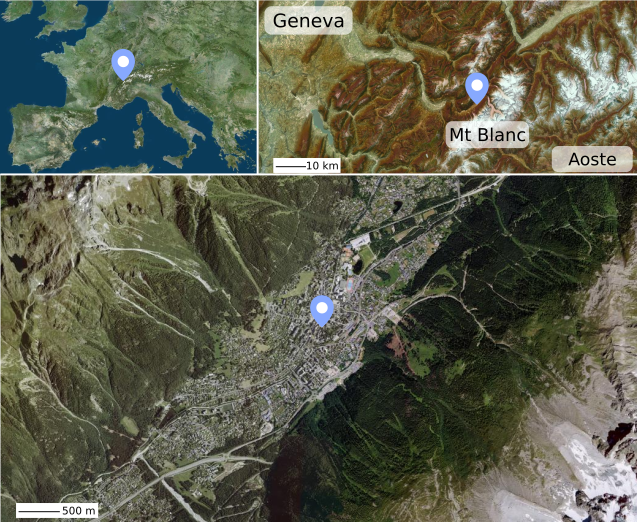
\includegraphics[width=8.3cm]{figures/fig01.png}
    \caption{Localisation of the sampling site in Chamonix, in the Arve Valley,
    France (45\unit{^\circ}55.358\unit{^\prime}~N,
6\unit{^\circ}52.194\unit{^\prime}~E).  $\copyright$~Planete observer, IGN}
    \label{fig:cham}
\end{figure}

\subsection{Chemical analyses }\label{chemical-analyses}

All filters were analysed using a large array of methods for the quantification
of chemical species including those important for the mass balance of the PM
(EC, OC, ions\ldots{}) and many organic and inorganic tracers of emission
sources. Briefly, the elements and components analyzed are:

\begin{itemize}
\item
  Organic and elemental carbon (OC, EC), using a Sunset instrument and
  the EUSAAR2 protocol \citep{aymoz_evolution_2004,cavalli_european_2016};
\item
  soluble anions and cations (NO\textsubscript{3}\textsuperscript{-},
  SO\textsubscript{4}\textsuperscript{2-}, Cl\textsuperscript{-} and
  NH\textsubscript{4}\textsuperscript{+}, Mg\textsuperscript{2+},
  Na\textsuperscript{+}, Ca\textsuperscript{2+}, K\textsuperscript{+})
  through ionic chromatography \citep{waked_source_2014};
\item
  inorganic elements (Al, Fe, Ti, As, Ba Cd, Ce, Cr, Cu, La, Li, Mn, Mo,
  Ni, Pb, Rb, Sb, Sn, Sr, V, Zn and Zr) using ICP-MS \citep{waked_source_2014};
\item
  sugar alcohols (arabitol, sorbitol, and mannitol, also called polyols)
  and anhydrous monosaccharides (levoglucosan, mannosan and galactosan)
  using an HPLC-PAD method \citep{waked_source_2014};
\item
  polar and nonpolar organic tracers (alkanes, hopanes, methoxyphenols,
  and substituted derivatives (methyl-PAHs) and polycyclic aromatic
  sulfur heterocycles (PASHs) using GC-MS and polycyclic aromatic
  hydrocarbons (PAHs) using HPLC-fluorescence \citep{golly_large_2015}.
\end{itemize}

Additionally, Black Carbon (eBC) measurements and the split between
biomass-burning BC\textsubscript{bb} and fossil-fuel BC\textsubscript{ff} were
maintained during the whole year with an Aethalometer model AE33
\citep{sandradewi_using_2008}. All the procedures for these chemical analyses
are described in detailed in \citet{chevrier_chauffage_2016}.

\subsection{\texorpdfstring{Source apportionment of PM\textsubscript{10}}{Source
apportionment of PM10}}\label{source-apportionment-of-pm10}

The source apportionment was achieved with Positive Matrix Factorization, using
the US EPA software PMF 5.0 \citep{us_epa_positive_2017}, following the
recommendations included in the european guideline book issued in the EU Fairmode program
\citep{belis_european_2014}. However, in the environment of Alpine valleys, the
local meteorology and frequent inversion layers in winter lead to strong
covariations of the concentrations of many chemical species emitted from the
valley bottom. Therefore, we developed an approach including several
specificities rarely applied in classic source apportionment in order to
overcome this problem in the PMF resolution \citep{chevrier_chauffage_2016}.

First, many tracers were included as input parameters, including specific
organic tracers. The benefit of such approach was previously described
\citep{golly_etude_2014,srivastava_speciation_2017,waked_source_2014}. In our
case, we included hopanes (thereafter named HOP), methoxyphenols, polyols (sum
of mannitol, arabitol and sorbitol), levoglucosan and MSA (methane sulfonic
acid). The OC is then replaced by OC* which is the difference between the OC and
the carbon equivalent of these species.

Second, elemental carbon (EC), which is an important species for the
deconvolution of combustion sources was replaced by
BC\textsubscript{bb} and BC\textsubscript{ff} obtained by concurrent
measurements with the Aethalometer model AE33. This provides a very strong
information on the sources, as already pointed out in other studies
\citep{petit_two_2015}. No correction was introduced to compensate between EC
and eBC \citep{zanatta_european_2016}.

Finally, we took advantage of the possibilities of PMF 5.0 to apply some
constraints to the factor profiles, in order to better define the sources
\citep{golly_etude_2014,srivastava_speciation_2017,salameh_impacts_2015}. A minimal set
of geochemically sounded chemical constraints based on prior and external
information of the source fingerprints was applied:
\begin{itemize}
    \item
        in the biomass burning factor, the contributions of levoglucosan, potassium,
        methoxyphenols and BC\textsubscript{bb} were pulled up maximally,
        whereas the BC\textsubscript{ff} and HOP were set to 0,
    \item
        HOP was pulled up maximally in the vehicular factor.
\end{itemize}

Table~\ref{tab:PMFentry} sums up the input chemistry species and respective uncertainties
used in the PMF study.
\begin{table*}
    \centering
    \caption{Selection of the chemical species used as input variables in the EPA PMF5.0
        model and their relative uncertainties. $\Sigma$polyols refers to the sum of
        arabitol, sorbitol and mannitol and $\Sigma$methoxyphenol to the sum of the
        particulate methoxyphenols.  The uncertainties in ``\%'' are relative to
        the sample concentration for the species.}
    \begin{tabularx}{\textwidth}{Xlccm{2.7cm}m{1.5cm}m{2.6cm}m{3cm}}
        \tophline
        & Total & \multicolumn{2}{c}{Carbonaceous matter} & Ions &
        \multicolumn{2}{c}{Organics compound} & Metals\\
        \middlehline
        Specie & PM\textsubscript{10} & OC* &
        BC\textsubscript{bb}, BC\textsubscript{ff} & Cl\textsuperscript{-},
        NO\textsubscript{3}\textsuperscript{-},
        SO\textsubscript{4}\textsuperscript{2-}, Na\textsuperscript{+},
        NH\textsubscript{4}\textsuperscript{+}, K\textsuperscript{+},
        Mg\textsuperscript{2+}, Ca\textsuperscript{2+} &
        $\Sigma$polyols, MSA,\newline levoglucosan &
        $\Sigma$HOP, $\Sigma$Methoxyphenol &
        As, Cu, Fe, Mn, Mo, Ni, Pb, Rb, Sb, Ti, V, Zn, Zr
        \\
        Uncertainty & 20\% & 10\% & 20\% & \citet{gianini_source_2013} &
        15\% & \citet{gianini_source_2013} & 2$\times$\citet{gianini_source_2013} \tabularnewline
        \bottomhline
    \end{tabularx}
    \label{tab:PMFentry}
\end{table*}


\subsection{Measurements of the Oxidative Potential of
PM}\label{measurements-of-the-oxidative-potential-of-pm}

All conditions are described in detail in \citet{calas_importance_2017}. In
brief, we performed the extraction of the PM in a simulated lung fluid (SLF)
solution to simulate the bio-accessibility of the PM and to be closer to the
exposure conditions. The extraction took place with the same amount of PM by
mass for each sample (at 10~\unit{\mu g~mL^{-1}}), by adjusting the area of filter
extracted. Samples were processed using the AA and DTT assays. DTT depletion
when in contact with PM extracts was determined by dosing the remaining amount
of DTT with DTNB (dithionitrobenzoic acid) at different reaction times and at
412~\unit{nm} using a plate spectrophotometer (Tecan, M200). The AA assay is a
simplified version of the synthetic respiratory tract lining fluid (RTFL) assay
\citep{kelly_protein_2003}, where only AA is used. AA depletion is read
continuously for 30~\unit{min} at 265~\unit{nm} (TECAN, 200). The maximum depletion rate of AA
is determined by linear regression of the linear section data. For both assays,
the 96-wells plate is auto shaken for 3 seconds before each measurement and kept
at 37~\unit{^\circ C}.

Only 98 samples out of the 115 collected were measured for OP, removing samples
with insufficient PM mass concentration (\textless{}5~\unit{\mu g~m^{-3}}) that did
not afford filter extraction at 10~\unit{\mu g~mL^{-1}}. The oxidative potential
(OP) unit is then expressed in nmol per minute per microgram of PM. However, the
population exposition is proportional to the inhaled PM. Therefore, the OP per
microgram is multiplied by the total mass of PM per cubic meter in order to
express the OP unit in \unit{nmol~min^{-1}~m^{-1}}. We should however keep in mind
that this measurement of OP may not be the exact OP from PM inhaled by the
population, since we suppose a linear relationship between the OP per~\unit{\mu g}
of PM and the OP of the total amount of PM. Indeed, some cocktail effects
like complexation or chelation may occur for PM concentrations higher than the
one tested. It has been shown by \citet{calas_importance_2017} that the result
is generally a probable over-estimation of the ``true'' OP. Hereafter, the OP
normalized by volume is denoted with a subscribed v (OP AA\textsubscript{v} and
OP DTT\textsubscript{v}).

\section{Results}\label{results}

\subsection{Evolution of the OP}\label{evolution-of-the-op}

As already mentioned in \citet{calas_importance_2017}, both assays present a strong seasonality
(see Figure~\ref{fig:OPts}) and both the OP AA\textsubscript{v} and OP
DTT\textsubscript{v} results follow a yearly cycle. The
OP\textsubscript{v} remains high during winter and low during summer.
This observation tends to emphasize the importance of the PM sources
which also follow a yearly cycle. However, we can also observe fast
variations from day to day, that may be related to a change in the PM
chemistry or to a change in PM concentration related to sources or
meteorological conditions.

Despite both assays following the same annual trend, some significant
differences exist. For instance, during summer, OP DTT\textsubscript{v}
has some activity whereas the values of OP AA\textsubscript{v} are close
to 0. Moreover, the variation of the OP AA\textsubscript{v} seems
smoother than that of OP DTT\textsubscript{v}, especially during summer
and fall (May to November). This underlines that the assays are
sensitive to different ROS.

\begin{figure*}[h]
    \centering
    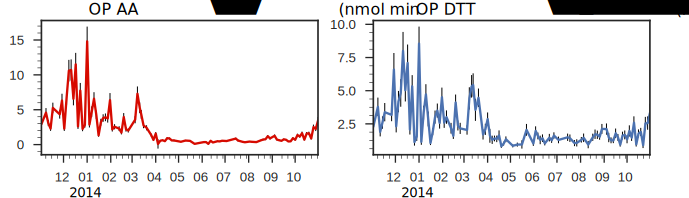
\includegraphics[width=\textwidth]{figures/fig02}
    \caption{OP AA\textsubscript{v} and OP DTT\textsubscript{v} variation from
        02 November 2013 to 31 October 2014 (98 samples) at the Chamonix station. The error
        bars represents the uncertainties (standard deviation) of the
        measurement. The OP unit is normalized by volume and is expressed
        in~\unit{nmol~min^{-1}~m^{-3}}.  }
    \label{fig:OPts}
\end{figure*}

\subsection{Evolution of the sources contributions}\label{evolution-of-the-sources-contributions}

The PMF was already thoroughly discussed in \citet{chevrier_chauffage_2016}. Briefly, 8
sources were identified: biomass burning, crustal dust, nitrate rich,
sulfate rich, primary and secondary biogenic emissions, salt and
vehicular emissions. Their respective main chemical species and related
information are provided in the Supplementary Information (SI 1). We
mainly see that metals (notably copper) and some organics species are
highly correlated to both OP, together with many fractions of the
carbonaceous matter (OC, BC\textsubscript{bb} and BC\textsubscript{ff}, see SI 2).
Figure~\ref{fig:PMFsrc} presents sources contributions to PM. Briefly, the dominant PM
source is biomass burning during winter with some daily concentrations
greater than 40~\unit{\mu g~m^{-3}}. The primary and secondary
biogenic sources are mainly active during summer, as is the sulfate
rich one. The vehicular source is quite constant all over the year. The
crustal dust contribution is sporadic and could include some Saharan
episodes \citep{aymoz_evolution_2004}. Finally, the salt source is low but
presents a high spike during March, being maybe related to road salting
at that time of the year. The correlation between the OP and the sources
are presented and discussed in the SI 2. Briefly, the Vehicular and
Biomass burning sources appears strongly correlated to both OP.

\begin{figure*}[h]
    \centering
    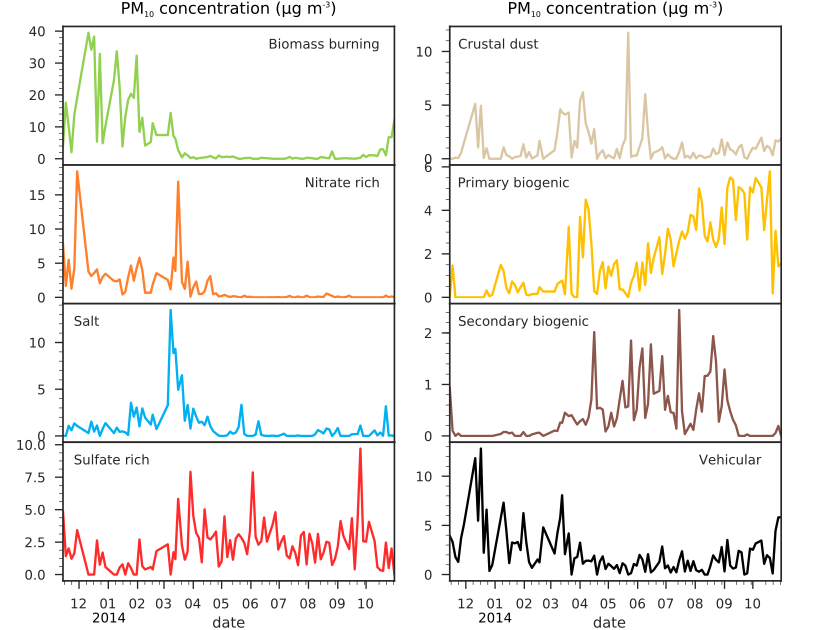
\includegraphics[width=\textwidth]{figures/fig03}
    \caption{Mass contribution of the eight PMF sources to the
    PM\textsubscript{10} from 14 November 2013 to 31 October 2014 (107 samples) at the
Chamonix station. Units are expressed in~\unit{\mu g~m^{-3}}.}
    \label{fig:PMFsrc}
\end{figure*}

\subsection{Setting up a multiple linear
regression}\label{setting-up-a-multiple-linear-regression}

As the OP is a value of reactivity, it cannot be directly introduced in
a mass-balance model. Hence, in order to estimate the contributions of
the PM emissions of sources to the OP, we must use an inversion
method. Despite the possible non linearity of OP values with increasing
masses of PM, as discussed below, we assume in this work that the OP is
linearly linked to the mass. Thus, we hereafter assume that OP and the
explanatory variables, namely the mass of the PM sources
m\textsubscript{PM}, are linearly related as follows
\begin{equation}
    \text{OP}_{\text{obs}} = m_{\text{PM}} \cdot \beta + \varepsilon
    \label{eq:sys}
\end{equation}
where OP\textsubscript{obs} is the ($n\times1$) observed OP matrix in~\unit{nmol~min^{-1}~m^{-1}}, m\textsubscript{PM} the ($n\times(p+1)$)
matrix with the PM mass attributed to each source expressed in~\unit{\mu g~m^{-3}} and a constant unity term with no unit
for the intercept, and $\varepsilon$ the ($n\times1$) uncertainty matrix in~\unit{nmol~min^{-1}~m^{-1}}; n is the number of observations and
p the number of sources. The estimator $\beta$ (matrix $(p+1)\times1$) represents
the intrinsic OP of the sources (i.e. the OP per mass unit of PM
attributed to a given source) and the intercept, expressed respectively
in~\unit{nmol~min^{-1}~\mu g^{-1}} for the intrinsic OP and in~\unit{nmol~min^{-1}~m^{-1}} for the intercept.

The optimal approximation of a solution for the linear system expressed
by equation \ref{eq:sys} is typically found by least squares. A variety of
methods exist differing on the function to be minimized and on the
regularization or sparsity penalty imposed to perform variable selection
on $\beta$, from ordinary least squares to ridge regression and LASSO (least
absolute shrinkage and selection operator). Here we have chosen a
Weighted Least Squares (WLS) approach as it has an integrated way to
handle the OP uncertainties. We have also chosen not to add a penalty
function as we do not have prior knowledge on the intrinsic OP values.
However, regular WLS do not rule out negative solutions, which should be
implemented in our case since it is not demonstrated that intrinsic OP
negative values exist in the real world. Therefore, a stepwise
regression is conducted. The underlying algorithm is

\begin{enumerate}
    \item
        Solve the WLS problem and estimate the intrinsic OP
    \item
        If an intrinsic OP is negative, then set it to zero and go back to step 1
    \item
        Repeat until all intrinsic OPs are positive or zero
\end{enumerate}

No source is discarded based on its p-value but only if its intrinsic OP
is negative. We did not choose a direct non-negative least square
approach as it would be a strong constraint in the model. In addition,
we can use the absence of negative coefficients as a test for the
coherence of our dataset. Indeed, such approach may allow us to
investigate which sources present a negative OP and why. This loop
converges in a finite number of iterations, either to a situation with
zero sources -- which would be discarded as absurd, pointing to a
breakdown of the underlying assumptions, or to an acceptable solution
with a lower number of sources. In our particular case, since OP
measurements never display negative values or negative source
contributions from the PMF, the method is strictly guaranteed to
converge to an acceptable solution. Further, we expressly do not set the
intercept to zero in equation \ref{eq:sys}, choosing instead to use this as a
check on our method. Indeed, if the system is well constrained (i.e. no
missing sources) the intercept should be close to zero within the model
uncertainties, without any explicit constraint. The reciprocal situation
could point to missing explanatory variables.

The uncertainties of the intrinsic OP are extracted from the variance of
$\beta$, which in turn is derived from the Hessian matrix of the WLS
regression in the standard way. However, the uncertainties on the
modelled OP are not analytically computed. Indeed, some coefficients
present co-variation due to the activity of the sources in the very same
period of the year, so analytical variance cannot be used to estimate
uncertainties. Therefore, in order to estimate the uncertainties of the
modelled OP, we bootstrap the solution $\beta$ 1000 times with a Monte-Carlo
algorithm. The bootstrap simply selects randomly an intrinsic OP for
each source according to their respective normal distribution.

The algorithm was implemented in Python 3 making use of the
\emph{statsmodels} WLS module \citep{seabold_statsmodels:_2010}.

\subsection{Application to the Chamonix site and
discussion}\label{application-to-the-chamonix-site-and-discussion}

Figure~\ref{fig:TSobsvsmodel} shows the comparison between observed and modelled OPs for the
measurements at the Chamonix site for both OP AA and OP DTT assays.
Table~\ref{tab:OPi} presents the intrinsic OP AA and OP DTT in~\unit{nmol~min^{-1}~\mu g^{-1}} for each
source with their respective uncertainties and p-values.

\subsubsection{Accuracy of the model}\label{accuracy-of-the-model}

The method developed in this study appears to be sufficiently accurate
to explain the two OP annual series at Chamonix. First, the seasonal
trend of the OP is very well reproduced, despite some under-estimation
of some of the highest values in winter. Second, the intercept of the
equation regression for OP AA\textsubscript{v} is not significant
(p\textgreater{}0.05). It is not so clear for the DTT test, but the
p-value remains high (p=0.04). We can consider the intercepts of the
equation regression as nearly negligible (see Table~\ref{tab:OPi}). The PM sources
presented in this study are then sufficient to explain the observed OP
AA\textsubscript{v} and OP DTT\textsubscript{v} time series. We can also
note that none of the sources was excluded for the DTT assay during the
inversion procedure due to negative contributions. It emphasizes the
fact that the sources explain well the observed OP. However, one source
was discarded for the AA assay: the crustal dust. Its p-value was less
than~0.01 for an intrinsic OP of $-0.05\pm$0.01~\unit{nmol~min^{-1}~\mu g^{-1}}. We supposed that the
crustal dust source in this study is a mixing of several sources,
including Saharan dust and road suspension dust. We could then end-up
with a mixing of highly different redox-active compounds towards AA test
that could explain the error for this source. Further work is needed to
understand this behavior.

\subsubsection{Uncertainties and residual}\label{uncertainties-and-residual}

The uncertainties of the modeled OP are quite low and mostly in the range of the
measurement uncertainties (Figure~\ref{fig:TSobsvsmodel}). Indeed, the
distribution of the residual is close to the normal law
(Figure~\ref{fig:residual}).  However, we can note an asymmetry toward
underestimation and residual seem to increase almost linearly with the
endogenous variable (no random repartition around 0 for the highest OP). The OP
is underestimated by the model for these high concentrated days. It may suggest
either non-linearity with high loading (as suggested above), or particular event
that is not apportioned by the sources provided in this study.

\begin{figure*}[h]
    \centering
    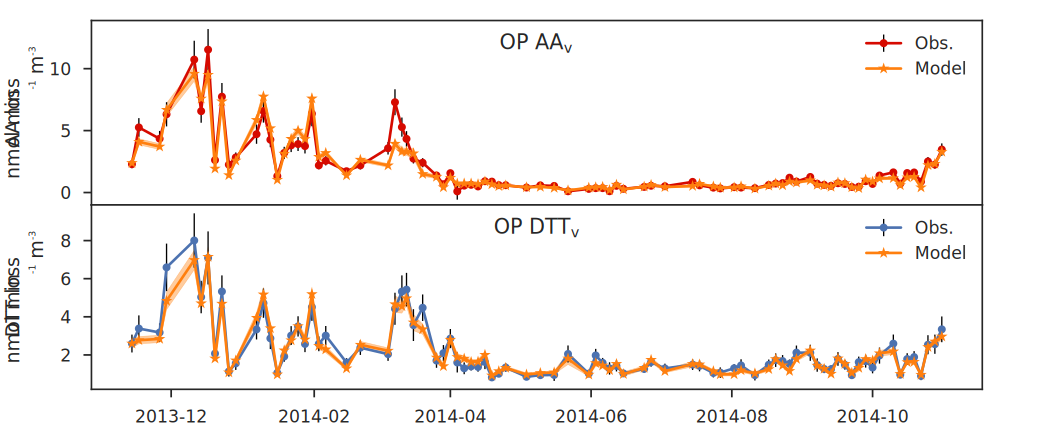
\includegraphics[width=\textwidth]{figures/fig04}
    \caption{Comparison of the modelled OP (orange) and the observed OP for both
        the AA (top graph) and DTT (bottom graph) test (85 samples) from
        November 2013 to November 2014. The black error bars are the standard
        deviation of the observed values and the shaded orange area the
    uncertainties of the modelled OP.  Units are in OP normalized by volume
    and expressed in~\unit{nmol~min^{-1}~m^{-1}}.}
    \label{fig:TSobsvsmodel}
\end{figure*}

\begin{figure}[h]
    \centering
    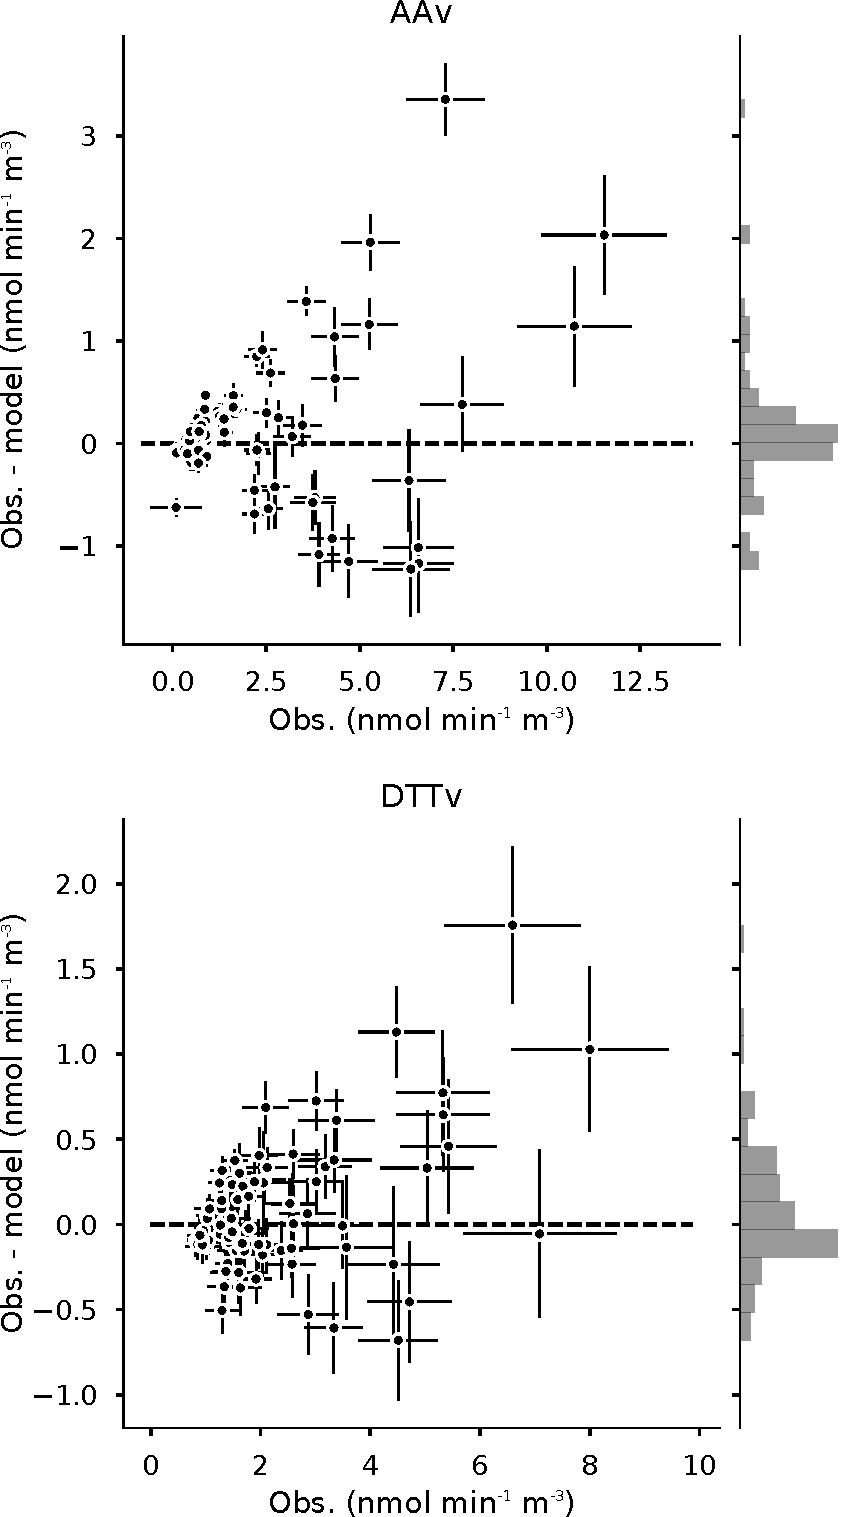
\includegraphics[width=8.3cm]{figures/fig05_v}
    \caption{Residual distribution for the regression of the AA and DTT assays
        (85 samples). The error bars represent the standard deviation of the
        observation and the model. The histogram on the right is the
        distribution of the residuals. Units are in OP normalized by volume and
        expressed in~\unit{nmol~min^{-1}~m^{-1}}.}
    \label{fig:residual}
\end{figure}

\subsubsection{Intrinsic OP}\label{intrinsic-op}

Values of the intrinsic OP of different sources for both the AA and DTT assays
are ranging from zero to 0.18$\pm$0.01~\unit{nmol~min^{-1}~\mu g^{-1}} for the AA test and from
0.06$\pm$0.02~\unit{nmol~min^{-1}~\mu g^{-1}} to 0.27$\pm$0.03~\unit{nmol~min^{-1}~\mu g^{-1}} for the DTT test
(Table~\ref{tab:OPi}). The various sources do not have the same ability to generate ROS. We also
note that the two tests present different intrinsic OP for the same source, and
the relative importance of the sources differs from one test to the other. For
instance, the vehicular source displays a lower intrinsic OP (0.15~\unit{nmol~min^{-1}~\mu g^{-1}})
than the biomass burning (0.18~\unit{nmol~min^{-1}~\mu g^{-1}}) for the AA test but a higher
intrinsic OP for the DTT test (0.27~\unit{nmol~min^{-1}~\mu g^{-1}} for the vehicular and
0.07~\unit{nmol~min^{-1}~\mu g^{-1}} for the biomass burning).  This deconvolution method may be
able to account for the chemical specificity of the two OP assays. In addition,
the DTT test seems to be more multi-sources influenced than the AA test.

Nevertheless, we clearly see the importance of the vehicular source, which is
associated to a strong intrinsic OP in both the AA and DTT assays. Previous
studies \citep{bates_reactive_2015,fang_oxidative_2016,verma_reactive_2014} also
highlighted the importance of this source to explain the OP AA and DTT. We may
explain such high intrinsic OP by the presence of metals in this source
-- notably the copper \citep{charrier_oxidant_2015}.

In the AA assay, the biomass burning also presents a high redox-activity
per~\unit{\mu g} of PM. This result disagrees with \citet{fang_oxidative_2016} as they found no
activity for this source in the OP AA test. Such difference for the biomass
burning source may be explained by the two extraction protocols (in water or in
a SLF solution) or by the proximity of the biomass source in Chamonix compared
to the longer distance transport in Atlanta, that would change the chemistry of
the source profile. However, the biomass burning in the OP DTT test has an
intrinsic OP of 0.07$\pm$0.01~\unit{nmol~min^{-1}~m^{-1}}, which is coherent
with the previous study of \citet{fang_oxidative_2016}. The presence of
oxygenated compounds such as quinones which are redox-active in the organic
matter could explain this high intrinsic OP.

The nitrate-rich source also appears to contribute in the redox-activity in both
assays. Although the nitrate itself is not redox-active, it can be co-emitted
with species that are oxidants. More work is needied in order to understand the
evolution of intrinsic OP for the nitrate rich factor, including measurements on
series characterized by specific spring events related to agricultural activities, and
series close to traffic sites for NO\textsubscript{x} emissions.

The Primary biogenic source, mainly identified by the presence of polyols,
presents a significant intrinsic OP. This result was unexpected. Indeed,
\citet{liu_therapeutic_2010} shows that mannitol is a strong anti-oxidant. Our
result suggests that some chemical species, present in the primary biogenic
source but not measured in this study, may contribute to the OP of the PM from
this source. Recently, it was shown that fungal spores exhibit a significant
intrinsic OP \citep{samake_unexpected_2017}, and this may be an hypothesis to be
further tested. However, the PMF profile of the primary biogenic source may also
be a mixing of different sources in our study (there is BC\textsubscript{ff} in
it for instance). Such mixing may also explain the high intrinsic OP of this
source.

\begin{table*}
    \centering
    \caption{Regression coefficients (i.e. Intrinsic OP) expressed in~\unit{nmol~min^{-1}~\mu g^{-1}} at Chamonix for the AA and DTT assays. The values are
        the mean$\pm$standard deviation based on N=1000 bootstrap of the best
        solution. The p-value is in the parenthesis. The Dust source was excluded during the inversion process for the AA
        test.}
        \begin{tabularx}{\textwidth}{lXXXXXXXXp{2.2cm}}
        \tophline
        & Biomass\newline burning & Crustal\newline dust & Nitrate\newline  rich & Primary\newline biogenic & Salt & Secondary\newline  biogenic &
        Sulfate\newline rich & Vehicular & Intercept\\
        \middlehline
        Unit & \multicolumn{8}{c}{\unit{nmol~min^{-1}~\mu g^{-1}}} & \unit{nmol~min^{-1}~m^{-1}}\\
        \middlehline
        AA & 
        0.18$\pm$0.01\newline (0.000) & -\newline (-) &
        0.12$\pm$0.02\newline (0.000) & 0.07$\pm$0.01\newline (0.000) &
        0.03$\pm$0.01\newline (0.140) & 0.02$\pm$0.04\newline (0.598) &
        0.00$\pm$0.01\newline (0.942) & 0.15$\pm$0.02\newline (0.000) &
        0.05$\pm$0.08\newline (0.502)\\
        DTT & 
        0.07$\pm$0.01\newline (0.000) & 0.07$\pm$0.02\newline (0.003) &
        0.07$\pm$0.02\newline (0.001) & 0.12$\pm$0.02\newline (0.000) &
        0.14$\pm$0.03\newline (0.000) & 0.18$\pm$0.05\newline (0.000) &
        0.06$\pm$0.02\newline (0.001) & 0.27$\pm$0.03\newline (0.000) & 
        0.17$\pm$0.08\newline (0.045)\\
        \bottomhline
    \end{tabularx}
    \label{tab:OPi}
\end{table*}

\subsubsection{Contribution to the OP}\label{contribution-to-the-op}

Due to the different intrinsic OP of the sources, the source contributions to
the OP (intrinsic OP times by the source contribution in~\unit{\mu g~m^{-3}}) is different from their contribution to the PM
mass.  Figure~\ref{fig:contributions} illustrates the normalized contribution of
the sources to the mass of the aerosols and the OP measures with AA and DTT. It
shows that the Vehicular source barely contributes to 17~\% of the total PM mass
during March-April-May (MAM) and June-July-August (JJA) but more than 30~\% to
the OP DTT\textsubscript{v} in the same period, and even reaching around 50~\%
of the OP AA\textsubscript{v} in JJA. Conversely, some sources largely
contributing to the PM\textsubscript{10} mass such as the sulfate-rich
source (30~\% of the total PM mass in JJA) do not contribute to the OP (2~\% to
the OP AA\textsubscript{v} in the same period). Finally, some sources like the
biomass burning contribute to a large extend in both PM mass and OP (on an
    annual basis: 35~\% of the PM mass, 55~\% of the OP AA\textsubscript{v} and
22~\% of the OP DTT\textsubscript{v}). We also note that on an annual basis, the
contribution of the Vehicular source is much larger for both OP assays than
for the mass.  All these outcomes are key parameters for policy initiatives.

To sum up, with this methodology, we observe a redistribution of the relative
importance of the sources ranked as ROS contributors. This study gives, and more
generally, the OP gives us a new vision of the atmospheric aerosols and
associated ROS burden. We also point out a clear distinction between the
different OP tests. Such differences raise new questions on OP assays choices
and standardization and require further investigation, especially coupled
OP-toxicology-epidemiology studies.

\begin{figure*}[h]
    \centering
    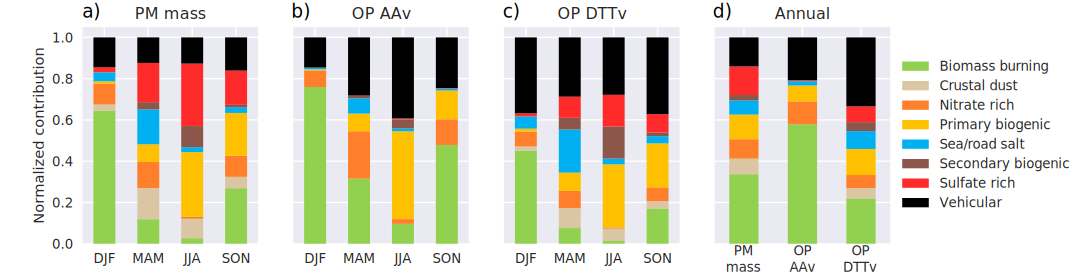
\includegraphics[width=\textwidth]{figures/fig06}
    \caption{Normalized seasonal contribution of the sources to a) the
    PM\textsubscript{10} total mass, b) the OP AA\textsubscript{v} and c) the OP
    DTT\textsubscript{v}. DJF is December-January-February, MAM is March-April-May,
JJA is June-July-August and SON is September-October-November. d) annual
normalized contributions of each source to the PM, OP AAv and OP DTTv.}
    \label{fig:contributions}
\end{figure*}

\section{Limitations}\label{limitations}

The method used in this study gives very good results and is promising for
practical application. However, since it has some limitations, we hereafter list
some possible improvements. First, as previously discussed, the model is
strongly constrained by the explanatory variable, which are the PM sources
contributions obtained with a PMF analysis. The PMF model has uncertainties of
two different natures, inherent to the model: 1) mathematical uncertainties on
the sources contributions and 2) frequent mixing profiles, due to co-linearity
induced, e.g., mainly by meteorology. In our study, we might encounter such
mixing for the biogenic sources. An improvement would be to bootstrap the PMF
results and use these uncertainties in the OP inversion in order to see its
sensitivity.

Another debatable choice is setting the intrinsic OP to zero for the source with
a negative intrinsic OP during the stepwise regression process. Some chemical
species may act as anti-oxidants which lead to ``negative'' intrinsic OP for the
associated PM source. Namely, the polyols from the Primary biogenic source, that
include species like mannitol, are known to present strong anti-oxidant
capabilities \citep{liu_therapeutic_2010} and bacteria can halve the OP of
copper-rich PM \citep{samake_unexpected_2017}. Further studies should focus on
this topic in order to better understand this potential effect.

Other choices of targets for optimization, and of penalty functions to promote
the positivity of the coefficients, are possible. However, we think that our
proposals manage to strike a balance between a satisfactory handling of the
uncertainties of the problem and ease of application using existing statistical
frameworks.


\conclusions  %% \conclusions[modified heading if necessary]

Based on one-year PM\textsubscript{10} sampling at an urban site located in
Chamonix (France) associated with chemical speciation and Oxidative Potential
(OP) measurements with the DTT and OP AA assays, we successfully established a
method to attribute the contribution of the PM sources to the observed OP.
The main conlusions of this study are summarized hereafter:
\begin{enumerate}
    \item
        The different sources present different OP AA and OP DTT per microgram of PM
        with intrinsic OP differences between sources up to a factor of 20.
    \item
        The Biomass burning and Vehicular sources seem to be the leading sources of
        the OP AA\textsubscript{v} and OP DTT\textsubscript{v} in Chamonix. On an
        annual basis, they represent together 78~\% of the OP AA\textsubscript{v} and
        54~\% of the OP DTT\textsubscript{v} apportionment.
    \item
        The two OP essays present different view on the PM sources based on their
        specific chemical selectivity as illustrated by the Salt source that does not
        contribute to the OP AA\textsubscript{v} but to the OP DTT\textsubscript{v}.
    \item
        The relative mass contributions of the sources to the PM\textsubscript{10}
        differ from their relative OP AA\textsubscript{v} and OP DTT\textsubscript{v}
        contributions. For instance, the vehicular source has a larger contribution to
        the total OP AA and OP DTT than to the total PM\textsubscript{10} mass,
        whereas the Sulfate rich source appears to be a minor source of OP
        AA\textsubscript{v} but an important source of PM mass. If OP is a proper
        metric of health impact of PM on population, the PM mass is not fully
        appropriate for PM regulations targeting public health.
\end{enumerate}

Finally, even if now, OP metric is correlated to health outcomes, this study
cannot directly attribute toxicity to one source or another. Is sporadic
exposure to PM with high OP values or chronical exposure to PM with low OP
values sufficient to provoke health damage?  As the DTT and AA tests point
different sources as the main ROS-generating, does one of them is the more
linked to toxicological effects (if any)? To answer these questions, more
cross-over studies including OP-epidemiology and toxicology are needed.












%% The following commands are for the statements about the availability of data sets and/or software code corresponding to the manuscript.
%% It is strongly recommended to make use of these sections in case data sets and/or software code have been part of your research the article is based on.

% \codeavailability{TEXT} %% use this section when having only software code available


% \dataavailability{TEXT} %% use this section when having only data sets available


% \codedataavailability{TEXT} %% use this section when having data sets and software code available





% \appendix
% \section{}    %% Appendix A
%
% \subsection{}     %% Appendix A1, A2, etc.
%
%
% \noappendix       %% use this to mark the end of the appendix section

%% Regarding figures and tables in appendices, the following two options are possible depending on your general handling of figures and tables in the manuscript environment:

%% Option 1: If you sorted all figures and tables into the sections of the text, please also sort the appendix figures and appendix tables into the respective appendix sections.
%% They will be correctly named automatically.

%% Option 2: If you put all figures after the reference list, please insert appendix tables and figures after the normal tables and figures.
%% To rename them correctly to A1, A2, etc., please add the following commands in front of them:

% \appendixfigures  %% needs to be added in front of appendix figures
%
% \appendixtables   %% needs to be added in front of appendix tables

%% Please add \clearpage between each table and/or figure. Further guidelines on figures and tables can be found below.



% \authorcontribution{TEXT} %% optional section

\competinginterests{The authors declare no conflict of intersest or competing
financial interests.} %% this section is mandatory even if you declare that no competing interests are present

% \disclaimer{TEXT} %% optional section

\begin{acknowledgements}
This work was funded in part by Primequal (DECOMBIO program in the Arve Valley,
grant ADEME 1362C0028) and by ANSES (ExPOSURE program, grant 2016-CRD-31). The
funding of the PhD for S.~Weber is provided by the Ecole Normale Sup\'{e}rieure.
The R\'{e}gion Auvergne Rh\^{o}ne-Alpes funded the PhD grant for F.~Chevrier. The
Universit\'{e} Grenoble Alpes funded the PhD grant of A.~Calas with a
Pr\'{e}sident Award. The funding of the post-doctoral position for D.~Salameh
comes from the SOURCES program (ADEME Grant 1462C0044). This study was also
supported by direct funding by IGE and LCME (technician salary), the LEFE CHAT
Potentiel oxydant program and the LABEX OSUG@2020 (ANR-10-LABX-56) (both for
funding analytical instruments).  ATMO AuRA conducted all the logistical aspect
of the sample collection in the field.

The authors would like to thanks Lisa Fluchaire, Jean-Charles Francony, Coralie
Conni\`{e}s, Vincent Lucaire, and Fanny Masson for their dedicated work for the
samples analyses, together with many people from Atmo AuRA for collection of
samples in the field. Many thanks also to Jesus Carrete Monta\~{n}a for fruitfully
improving the ideas in this work.
\end{acknowledgements}




%% REFERENCES

%% The reference list is compiled as follows:

% \begin{thebibliography}{}
%
% \bibitem[AUTHOR(YEAR)]{LABEL}
% REFERENCE 1
%
% \bibitem[AUTHOR(YEAR)]{LABEL}
% REFERENCE 2
%
% \end{thebibliography}

\bibliographystyle{copernicus}
\bibliography{bibtex}

%% Since the Copernicus LaTeX package includes the BibTeX style file copernicus.bst,
%% authors experienced with BibTeX only have to include the following two lines:
%%
%% \bibliographystyle{copernicus}
%% \bibliography{example.bib}
%%
%% URLs and DOIs can be entered in your BibTeX file as:
%%
%% URL = {http://www.xyz.org/~jones/idx_g.htm}
%% DOI = {10.5194/xyz}


%% LITERATURE CITATIONS
%%
%% command                        & example result
%% \citet{jones90}|               & Jones et al. (1990)
%% \citep{jones90}|               & (Jones et al., 1990)
%% \citep{jones90,jones93}|       & (Jones et al., 1990, 1993)
%% \citep[p.~32]{jones90}|        & (Jones et al., 1990, p.~32)
%% \citep[e.g.,][]{jones90}|      & (e.g., Jones et al., 1990)
%% \citep[e.g.,][p.~32]{jones90}| & (e.g., Jones et al., 1990, p.~32)
%% \citeauthor{jones90}|          & Jones et al.
%% \citeyear{jones90}|            & 1990



%% FIGURES

%% When figures and tables are placed at the end of the MS (article in one-column style), please add \clearpage
%% between bibliography and first table and/or figure as well as between each table and/or figure.


%% ONE-COLUMN FIGURES

%%f
%\begin{figure}[t]
%\includegraphics[width=8.3cm]{FILE NAME}
%\caption{TEXT}
%\end{figure}
%
%%% TWO-COLUMN FIGURES
%
%%f
%\begin{figure*}[t]
%\includegraphics[width=12cm]{FILE NAME}
%\caption{TEXT}
%\end{figure*}
%
%
%%% TABLES
%%%
%%% The different columns must be seperated with a & command and should
%%% end with \\ to identify the column brake.
%
%%% ONE-COLUMN TABLE
%
%%t
%\begin{table}[t]
%\caption{TEXT}
%\begin{tabular}{column = lcr}
%\tophline
%
%\middlehline
%
%\bottomhline
%\end{tabular}
%\belowtable{} % Table Footnotes
%\end{table}
%
%%% TWO-COLUMN TABLE
%
%%t
%\begin{table*}[t]
%\caption{TEXT}
%\begin{tabular}{column = lcr}
%\tophline
%
%\middlehline
%
%\bottomhline
%\end{tabular}
%\belowtable{} % Table Footnotes
%\end{table*}
%
%
%%% MATHEMATICAL EXPRESSIONS
%
%%% All papers typeset by Copernicus Publications follow the math typesetting regulations
%%% given by the IUPAC Green Book (IUPAC: Quantities, Units and Symbols in Physical Chemistry,
%%% 2nd Edn., Blackwell Science, available at: http://old.iupac.org/publications/books/gbook/green_book_2ed.pdf, 1993).
%%%
%%% Physical quantities/variables are typeset in italic font (t for time, T for Temperature)
%%% Indices which are not defined are typeset in italic font (x, y, z, a, b, c)
%%% Items/objects which are defined are typeset in roman font (Car A, Car B)
%%% Descriptions/specifications which are defined by itself are typeset in roman font (abs, rel, ref, tot, net, ice)
%%% Abbreviations from 2 letters are typeset in roman font (RH, LAI)
%%% Vectors are identified in bold italic font using \vec{x}
%%% Matrices are identified in bold roman font
%%% Multiplication signs are typeset using the LaTeX commands \times (for vector products, grids, and exponential notations) or \cdot
%%% The character * should not be applied as mutliplication sign
%
%
%%% EQUATIONS
%
%%% Single-row equation
%
%\begin{equation}
%
%\end{equation}
%
%%% Multiline equation
%
%\begin{align}
%& 3 + 5 = 8\\
%& 3 + 5 = 8\\
%& 3 + 5 = 8
%\end{align}
%
%
%%% MATRICES
%
%\begin{matrix}
%x & y & z\\
%x & y & z\\
%x & y & z\\
%\end{matrix}
%
%
%%% ALGORITHM
%
%\begin{algorithm}
%\caption{…}
%\label{a1}
%\begin{algorithmic}
%…
%\end{algorithmic}
%\end{algorithm}
%
%
%%% CHEMICAL FORMULAS AND REACTIONS
%
%%% For formulas embedded in the text, please use \chem{}
%
%%% The reaction environment creates labels including the letter R, i.e. (R1), (R2), etc.
%
%\begin{reaction}
%%% \rightarrow should be used for normal (one-way) chemical reactions
%%% \rightleftharpoons should be used for equilibria
%%% \leftrightarrow should be used for resonance structures
%\end{reaction}
%
%
%%% PHYSICAL UNITS
%%%
%%% Please use \unit{} and apply the exponential notation


\end{document}
